\documentclass[12pt]{paper}

\usepackage{Schwieg}
\usepackage[margin=1in]{geometry}
\usepackage{geometry}
\usepackage{tikz}

\title{ Problem Set 3 Question 2}
\author{ Timothy Schwieg \and Samuel Barker \and Rafeh Qureshi \and Daniel Noriega}

\begin{document}

\maketitle

\section*{Model}

In a very reduced-form manner, consider individuals that have some
demand for universities and $x^{*}( p_D, ... )$ for private
universities over public universities where $p_D$ is the
inflation-adjusted difference between tuition rates, and $...$ are all
other parameters that do not include the tuition ratio. Assume that
$x^{*}$ is decreasing in $p_D$. This means that as the difference
grows, individuals demand private education less than public
education. This is equivalent to assuming that private universities
have higher tuition rates than public universities, and the
substitution effect dominates the income effect for university
education. We can see that equal (after adjusting for inflation) absolute
changes in the tuition rates will not change $p_D$, and therefore not
change the demand of the private or public universities relative to the other. It is
possible however that total university demand may change.

\section{How would a proportional increase in the tuition of both
  types of schools affect the market share of public schools?}

A representative budget constraint for an individual would look like the following:

\begin{equation*}
  p_g g s + p_v (1-g) s + p_A A = M
\end{equation*}

Where $p_g$ is the price of public universities, $p_v$ is the price of
private universities, and $p_A$ is the price of all other goods lumped
into an auxiliary good.

For a proportional increase in the tuition of $\alpha$, the average price
level will increase by $\beta < \alpha$ as education spending is only a
portion of the overall budget. When we calculate the real tuition
rates for each country, then they will have increased by roughly
$\frac{1+\alpha}{1+\beta} > 1$ percent. 

If tuition costs of private and public universities were initially
$p_1$ and $p_2$ respectively, new prices would then be
$(1+\alpha) p_1$ and $(1+\alpha) p_2$. The inflation adjusted difference between
them would then be:
$ \left (\frac{1+\alpha}{1+\beta} \right ) ( p _1 - p_2 ) > p_1 - p_2$. This
tells us that the inflation adjusted difference is larger the bigger
the proportional increase in tuition. Since the relative demand of
public universities increases on the difference of tuition costs (see
model setup section), we conclude that the relatively cheaper option:
public universities, will then get a higher market share relative to
the initial state.


\section{Assuming that proportional tuition changes did change market
  shares, would this substitution effect be inconsistent with the
  homogeneity restriction from demand theory? }

No it is not inconsistent. Homogeneity is a property that involves the
entire vector of prices that the consumer faces as well as his
income. We must see an increase in all prices by the same amount as
well as the income of all individuals to evaluate homogeneity
properties. We have seen changes prices of only two goods which are
only a portion of an individuals' budget.  All that has happened is
that two goods have become relatively more expensive. In general there
is both a substitution and income effect when this occurs.

Alternatively, we could assume that students only have their education as the
only good in their world. Then the proportional increase in the
prices of the two goods would still not violate homogeneity, as
the income is not being increased by the same proportion.

\subsection{What if the household
  incomes also increased in the same proportion as tuition rates?}

Consider the case where consumers only value spending on
education. The only goods that the consumers consider buying are
attending either public or private universities. The inflation rate
could be assumed to be exactly the change in the tuition rates, as
they take up the entire basket share of goods. In this case, we would
see that $\frac{1+\alpha}{1+\beta} = 1$ so that the inflation-adjusted
difference between the tuition rates has not changed. Therefore there
would be no change to the market share of either type of
university. This means there is no violation of homogeneity.

If we believe that the market share is changing, then there must be
other goods in the consumers basket, and we would have to assume that
they have all increased in the same proportion. Otherwise, the entire
price vector $\vec{p}$ would not have changed proportionately and it
would not be possible to evaluate homogeneity properties.

\section{Is the quasilinear utility function below consistent with
  observations?}

\begin{equation*}
  u(g,s) = \delta s g - s g \log ( s g ) - (1-g)s \log( (1-g) s) + f(s) + s
  \log \left( \frac{s}{1 + \exp(\delta)} \right) - t_g g s - t_v (1-g)s
\end{equation*}

The question that the representative consumer faces is to maximize
this function subject to some budget constraint.

\begin{align*}
  \max_{g,s} \quad &u(g,s)\\
  \text{s.t}\quad & t_g g s + t_v s( 1- g) = M
\end{align*}

One important thing to notice is that this budget constraint appears
in the utility function, so we may apply it to simplify the utility
function partially.

We are interested in whether or not this utility function displays the
properties of individuals demand depending on the inflation-adjusted
difference between the prices of the universities rather than the
relative price. One way to model this is to change both of the prices
by the same fixed amount, and determine if the optimal market share
changes with this increase. If it does not, then they are making
choices based on the difference rather than the relative price. To
this end we add to the tuition prices a fixed amount of $\Delta$. However,
since the individuals only consume education, when the prices increase
by $\Delta$. Every individual has an increased expenditure of
$s \Delta$. We wish to hold real income constant while we adjust the
prices. To compensate for this inflation, we subtract this quantity to
the expenditures to ensure that there is a constant real income. The
consumer's problem has become:

\begin{align*}
  \max_{g,s} \quad &\delta s g - s g \log ( s g ) - (1-g)s \log( (1-g) s) +
                 f(s) + \\
  &\quad\quad\quad s \log \left( \frac{s}{1 + \exp(\delta)} \right) - M\\
  \text{s.t}\quad & (t_g+\Delta) g s + (t_v + \Delta) s( 1- g) - \Delta s = M
\end{align*}

After setting up the Lagrangian, We take the first order
conditions. The solutions to these first order conditions are the
functions $g^{*}, s^{*}$ and $\lambda^{*}$ that determine the optimal
choices for various parameters.

\begin{align*}
  0 &= s \left ( \delta + \lambda \left(t_{g} - t_{v}\right) - \log{\left (g s \right
  )} + \log{\left ( s \left(1-g\right) \right )}\right)\\
  0 &= g \delta - g \log{\left (g s \right )} + \lambda \left[ g \left(t_{g} +
  \Delta\right) - \Delta + \left(1-g\right) \left(t_{v} + \Delta\right)\right] +
      \left(g - 1\right) \log{\left [s \left(1-g\right) \right ]}\\
  & \quad \quad \quad + \log{\left (\frac{s}{e^{\delta} + 1} \right )} + f'\left (s \right )\\
  0 &= g s \left( t_g - t_v \right) - m + s t_{v}
\end{align*}

We are interested in whether or not $\deriv{g^{*}}{\Delta} = 0$. We shall
compute this value using the implicit function theorem, as we cannot
explicitly solve these first-order conditions. The solution for this
will be by using Cramer's rule.


The determinant of the Jacobian of this system is given by:

$$\abs{J} = \begin{vmatrix}
  \frac{s}{g \left( 1- g\right)} &
  \delta + \lambda \left(t_{g} - t_{v}\right) - \log{\left (g s \right )} + \log{\left ( s \left(1-g\right) \right )} &
  s \left(t_{g} - t_{v}\right)\\
  
  \delta + \lambda \left(t_{g} - t_{v}\right) - \log{\left (g s \right )} + \log{\left ( s \left(1-g\right) \right )} &
  - f''{\left (s \right )} &
  g t_{g} - g t_{v} + t_{v}\\
  
  s \left(t_{g} - t_{v}\right) &
  g t_{g} - g t_{v} + t_{v} &
  0
\end{vmatrix}$$

Applying Cramer's rule to obtain the value of $\deriv{g^{*}}{\Delta}$.


$$\abs{J_{\Delta}} = \begin{vmatrix}
  0 &  \delta + \lambda \left(t_{g} - t_{v}\right) - \log{\left (g s \right )} + \log{\left ( s \left(1-g\right) \right )} &  s \left(t_{g} - t_{v}\right)\\
  0 &  - f''{\left (s \right )} &  g t_{g} - g t_{v} + t_{v}\\  
  0 &  g t_{g} - g t_{v} + t_{v}&  0
\end{vmatrix} = 0$$

Since there is a column of all zero values, we can see that
$\abs{J_{\Delta}} = 0$. Since we know that $\abs{J} \neq 0$ as it is the
Hessian of the utility maximization problem. Using the implicit
function theorem we see that $\deriv{g^{*}}{\Delta} =
\frac{\abs{J_{\Delta}}}{\abs{J}} = 0$. This tells us that as the prices of
the education change, but the inflation-adjusted difference between
them remains constant, the market share does not change. This confirms
that this utility function is consistent with the above observations.

\section{How is the utility function above related to the logit demand
  model?}

Let us believe that the valuations for public and private education
are distributed Gumbel. These valuations are reduced by the inflation
adjusted prices of attending each university. We shall assume that the
scale parameters of both valuations are equal and normalized to $1$.

Allow for the location parameter for public education: $\mu_v = \delta - t_v$
and the location parameter for private education: $\mu_g = - t_g$ If the
tuition rates for each were equal, the valuations for private
education would be $\delta$ higher on average. 

The individual will choose to attend public university based on
whether or not the difference in the valuations is positive or
not. The difference of two Gumbel distributions is logistic. The
location parameter will be $\delta + t_g - t_v$ and the scale parameter
will remain normalized to $1$. The cdf is given by:
\begin{equation*}
  \frac{1}{1 + \exp \left( - ( x- \delta + t_g - t_v) \right)}
\end{equation*}

If this logistic random variable is positive, then the valuation for
the private education is higher than the valuation for the public
education. We can think of demand for private education by the
probability that this realization is positive, for a given set of
factor prices.

This probability is given by:
\begin{equation*}
  \Pr( V \leq 0) = \frac{\exp \left( t_g - t_v - \delta \right)}{\exp \left( t_g - t_v - \delta \right) + 1}
\end{equation*}

As the difference of the tuition rates
$t_g - t_v = - (t_v - t_g)$ increases, the cost premium, $t_v - t_g$
of private education decreases. This means that private education and
relatively cheaper. From the cdf we see that the probability of
purchasing private education increases as the cost premium decreases.

For a quasilinear utility function, the demand for a good depends only
on the prices and not on the income of the individual. This would
imply that for a demand function $x_i^{*}$, $\deriv{x_i^{*}}{M} =
0$. In the logit model, the probability that a student attends a
type of university times the number of students gives the demand
function for each type of university. Note that the probability of
attending a particular type of university does not depend on the
income of the student. It depends only on the preference of private
education $\delta$ and the difference in the tuition rates. This displays
the same properties of the quasilinear utility function in the
percentage of people attending the university.



\section{Other than the model(s) you used for (c) and (d), what is
  another way to model the dependence of market shares on price differences rather than ratios?}

Consider a world where private and public education are perfect
substitutes. If individuals are completely indifferent between
consuming education at a private or public university, they will
simply choose the university with the lowest price. In this case, the
demand function will be based on whether or not the difference between
the tuition rates is positive or negative. Absent other conditions,
all students will consume the cheapest alternative, either public or
private education. This is a strong form of substitution where one
unit of the private university is worth the same as one unit of the
public university (i.e. perfect substitutes with $\alpha = 1$).

Find below sample graphs of the demand functions against the inflation
adjusted difference in the prices $P_D$. 

\begin{figure}[h!]
  \centering
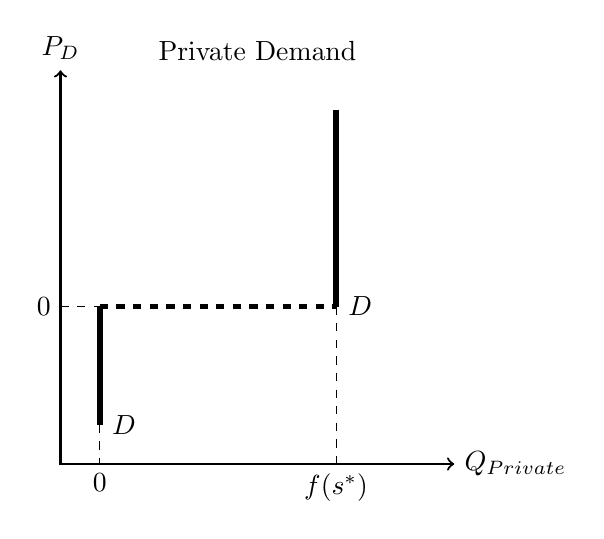
\begin{tikzpicture}[scale=0.5]

\draw[thick,<->] (0,10) node[above]{$P_{D}$}--(0,0)--(10,0) node[right]{$Q_{Private}$};

\node [left] at (0,4) {$0$};

\node [below] at (7,0) {$f(s^{*})$};
\node [below] at (1,0) {$0$};

\node [above] at (5,10){Private Demand};

\draw[line width=.75mm](7,9)--(7,4) node[right]{$D$};
\draw[line width=.75mm](1,4)--(1,1) node[right]{$D$};

\draw[dashed](7,4)--(7,0);
\draw[dashed](1,1)--(1,0);
\draw[dashed](0,4)--(1,4);
\draw[dashed, line width=.75mm](1,4)--(7,4);

\end{tikzpicture}
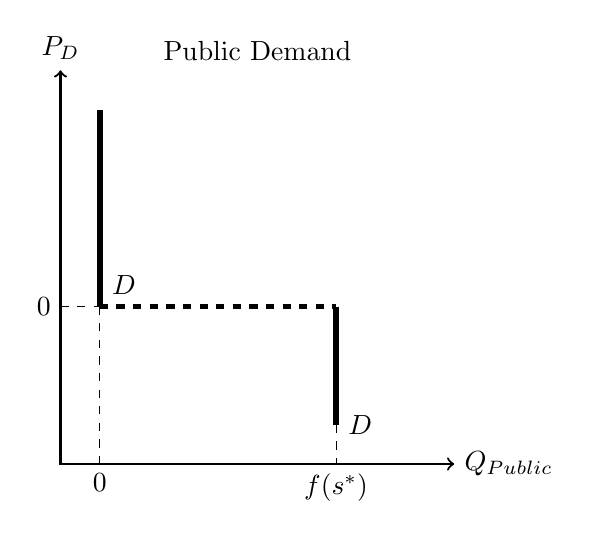
\begin{tikzpicture}[scale=0.5]

\draw[thick,<->] (0,10) node[above]{$P_{D}$}--(0,0)--(10,0) node[right]{$Q_{Public}$};

\node [left] at (0,4) {$0$};

\node [below] at (7,0) {$f(s^{*})$};
\node [below] at (1,0) {$0$};

\node [above] at (5,10){Public Demand};

\draw[line width=.75mm](7,4)--(7,1) node[right]{$D$};
\draw[line width=.75mm](1,9)--(1,4) node[above right]{$D$};

\draw[dashed](7,1)--(7,0);
\draw[dashed](1,4)--(1,0);
\draw[dashed](0,4)--(1,4);
\draw[dashed, line width=.75mm](1,4)--(7,4);

\end{tikzpicture}
\end{figure}

% One possible way to model this is to take an extremely reduced form
% approach against the structural approach used in $c$. If we assume
% that the demand for college is linear in income and tuition prices. We
% allow the market share to just be a function of only the price
% difference between the tuition. This reduced form approach assumes
% that there is an equilibrium in the background generating this demand
% system.

% \begin{align*}
%   s &= \alpha_1 + \beta_1 t_g + \gamma_1 t_v + \delta_1 M\\
%   g &= \min \{ \max \{ \phi ( t_v - t_g) + \upsilon, 0  \}, 1 \}
% \end{align*}

% This ensures that $g$ is between $0$ and $1$ and is thus a valid
% probability. The market share depends solely on the difference between
% the two utilities. It would be possible to assume a non-linear
% functional form instead of the linear demand, however the linear
% nature simplifies the model and allows for easier estimation.

% This method would assume that there was an equilibrium and utility
% maximization that was occurring in the background that led to this
% particular aggregate demand function for universities. This would be
% the simplest way to ensure that the demand behaved as we
% wished. However this would not be able to be used for any policy
% prediction, as it is victim to the Lucas Critique. Without a
% structural estimation, we cannot use this to model the effect of
% policy changes. If we were interested in examining how these would
% change under a new set of policies as in part $f$, we would need to
% estimate it structurally as in part $c$.

\section{If the federal government were considering whether its
  college tuition subsidies should be the same for all universities
  versus proportional to tuition, what are some of the reasons why
  private universities would favor the proportional subsidy? Are there any reasons why they would favor the constant
  subsidy?}

Let the market share of the public universities be given by
$g$. Assume that the university will spend its subsidy solely on
reducing tuition for its students. Also, assume that when subsidies
are said to be ``the same'' for all universities, it means that all
universities will get a subsidy of ``x dollars'' per student,
irrespective of the value of tuition. Similarly, when subsidies are
said to be ``proportional to tuition'', it means that universities will
receive a subsidy of ``x percent'' of tuition per student.

A proportional subsidy would effectively decrease the inflation
adjusted tuition cost difference, and therefore, the market share of
private universities would increase. In other words, private
universities would favor a proportional subsidy because since their
tuition costs are higher, they would perceive comparatively a higher
benefit.

Alternatively, we could assume that the subsidy amount is a fixed
quantity from the government perspective, and that the question is
only how it should be allocated. In this scenario, the effective
change in tuition costs would depend on the number of students in each
university in addition to the allocation mechanism. If the mechanism
was the ``same subsidy'' for either public or private school, there
would be two possibilities, which are described below:

\begin{itemize}
\item If private colleges have a smaller share of the market compared
  to public colleges, their effective subsidy (i.e. change in tuition
  per student) will be greater than the effective subsidy for public
  colleges. Therefore, private colleges' market share would increase.

\item If private schools have a larger market share than public
  colleges, the effective subsidy under the "same" mechanism would be
  less than the effective subsidy for public colleges. Therefore, the
  subsidy would actually decrease private colleges market share.
\end{itemize}

In short, private colleges would favor the "same subsidy" mechanism
under the fixed subsidy amount scenario when they have a smaller
market share than public colleges.
\\

Conversely, if the mechanism for allocating subsidies were the
``proportional subsidies'' under the fixed subsidy amount assumption,
there will be two additional scenarios, which are described below:

\begin{itemize}
\item If private colleges have a smaller share of the market, then
  they will ineluctably receive a higher effective subsidy. They would
  receive an bigger subsidy in absolute terms due to the higher
  tuition costs, but additionally the fact that their number of
  students is smaller would further increase the effective subsidy
  that private colleges receive compared to public
  schools. Consequently, private colleges' share of the market would
  increase.

\item If private colleges have a larger market share than public
  colleges, the effective subsidy under the ``proportional subsidies''
  would be uncertain. This occurs because even though the absolute
  subsidy that private colleges receive is larger due to the higher
  tuition costs, the actual effect is counter by the larger number of
  students. In particular, private colleges would favor this mechanism
  only when $\frac{1-g}{g} < \frac{t_v}{t_g}$. Where $t_v, t_g$ are
  the tuition as before.
\end{itemize}

In conclusion, under the fixed subsidy assumption, private colleges
will favor the proportional subsidy for certain when they have a
smaller market share than public colleges. If they had a larger market
share, private colleges' support in favor of the measure would depend
on the given conditions for tuition costs and market shares.


\end{document}
